\section{What the image fallback rejects}
\label{sec:fallback_raw_outputs}
The final client in Section~\ref{sec:fallback_failure} always returns an output that passes its frozen paired-content gates, because it can retain the supplied source generator and fall back to its output. This does not mean the raw adapted generator always preserves the source. The figure illustrates that distinction: left is the supplied source output, middle is the raw 500-update adaptation, and right is the returned quality-gated output. Source positions 0, 16, 32 and 48 are fixed by position after the run, without outcome filtering. All source, raw and returned PNG hashes and raw quality hashes are checked against the final artifact freeze. A failed raw adaptation remains visible even when the client returns the unchanged source.

Raw preservation requires all four gates: LPIPS at most $0.2$, SSIM at least $0.6$, image-image CLIP cosine at least $0.9$, and class-alignment retention at least $0.95$. A low LPIPS alone therefore does not imply a pass. The bit-accuracy labels are rounded for display; owner decisions use their full values and the frozen strict threshold $>0.6875$.

\begin{figure}[p]\centering
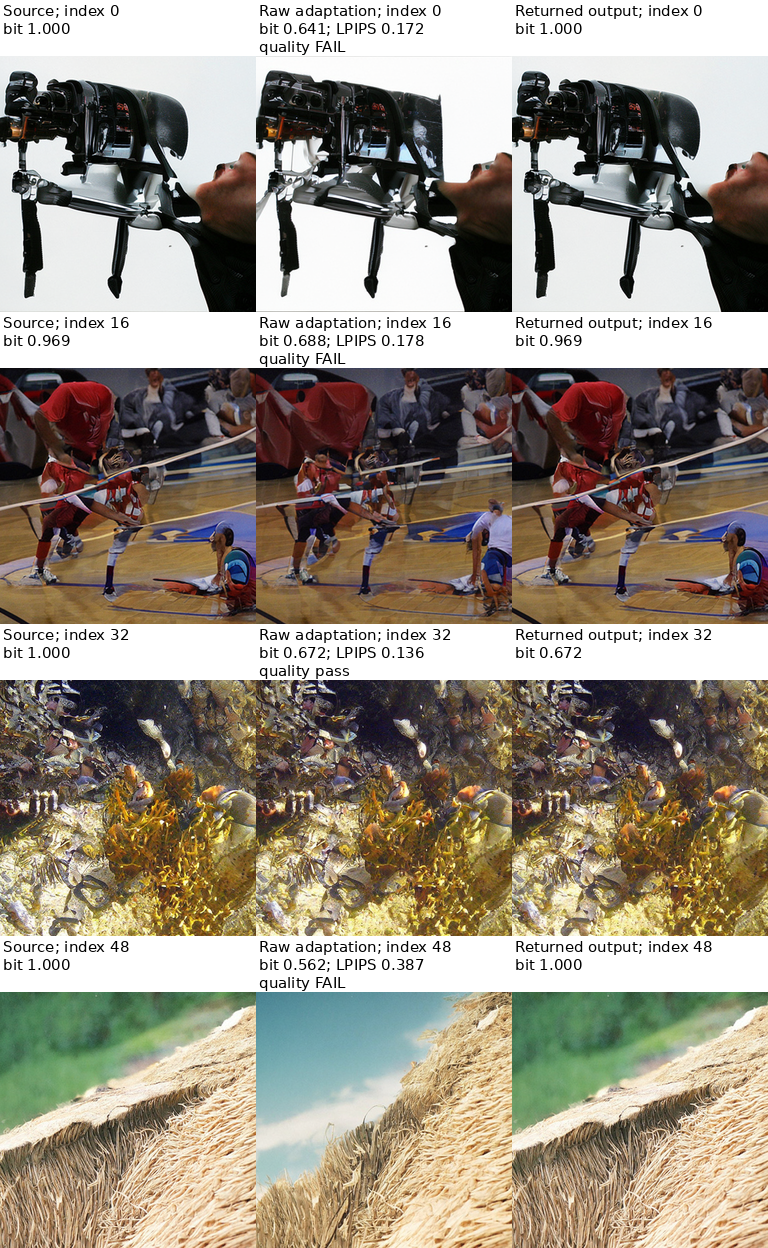
\includegraphics[width=.84\linewidth]{figures/preserving-fallback-triplets-original.png}
\caption{Released model: source, raw adaptation and returned output. LPIPS and the raw preservation decision are shown in the middle column. A low raw bit accuracy is insufficient for joint success if the content changes too much.}
\end{figure}

The fixed-target and adapted-target galleries use the same positions and are in \path{tex/figures/}.
